You have been provided a USB stick with all you will need for this tutorial. On
this drive is the following: ICE binaries for your OS, a clone of the ICE git
repository, all tutorial documentation and slides for today, and
data files for the tutorial. 

\section*{ICE Installation}
A number of files must first be copied from the
USB stick to your local machine:
\begin{enumerate}
\item Choose a location that is easy to remember
and copy the correct \texttt{ice\-product*.zip} file for your computer's 
operation system (Linux, Mac OS X, or Windows).
\item Unzip this file to obtain the 
ICE application executable.
\item Copy the git repository \texttt{repository.zip} file to your computer.
\item Unzip this file.
\end{enumerate}

\section*{Starting ICE}
To start ICE, double-click on the application executable to open up ICE. When the workspace chooser
dialog opens, select the default workspace. 
\begin{center} 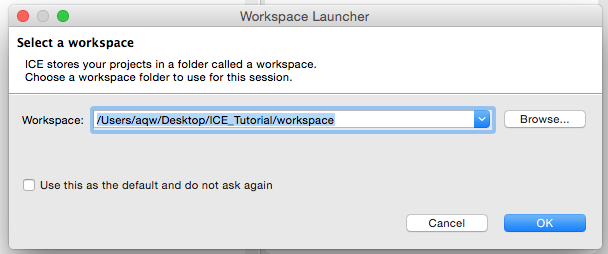
\includegraphics[width=\textwidth]{figures/workspace}
\end{center}
When ICE opens you should see something similar to the below image. 
\begin{center} 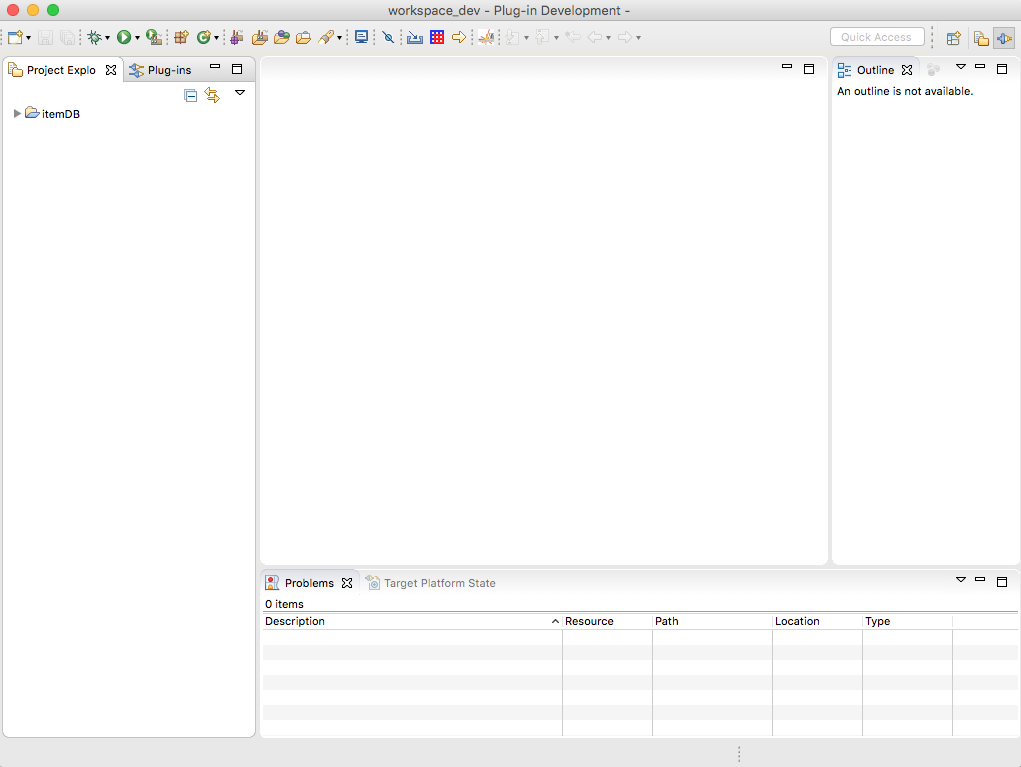
\includegraphics[width=\textwidth]{figures/expectedICE}
\end{center} 

\section*{Setting up ICE}
In order to develop an application dashboard, a development version of ICE
must be setup. The first step in doing this is to load the ICE bundles into
your workspace. We have provided a developer menu to assist in this process:

\begin{enumerate}
\item Select \texttt{Developer $\rightarrow$ ICE $\rightarrow$
Import from local repository}
\item Using the directory dialog, navigate to the git repository you copied
from the USB drive.
\item Select \texttt{Open}
\end{enumerate}

This should import all the ICE bundles and you should have something
like the image below.
\begin{center} 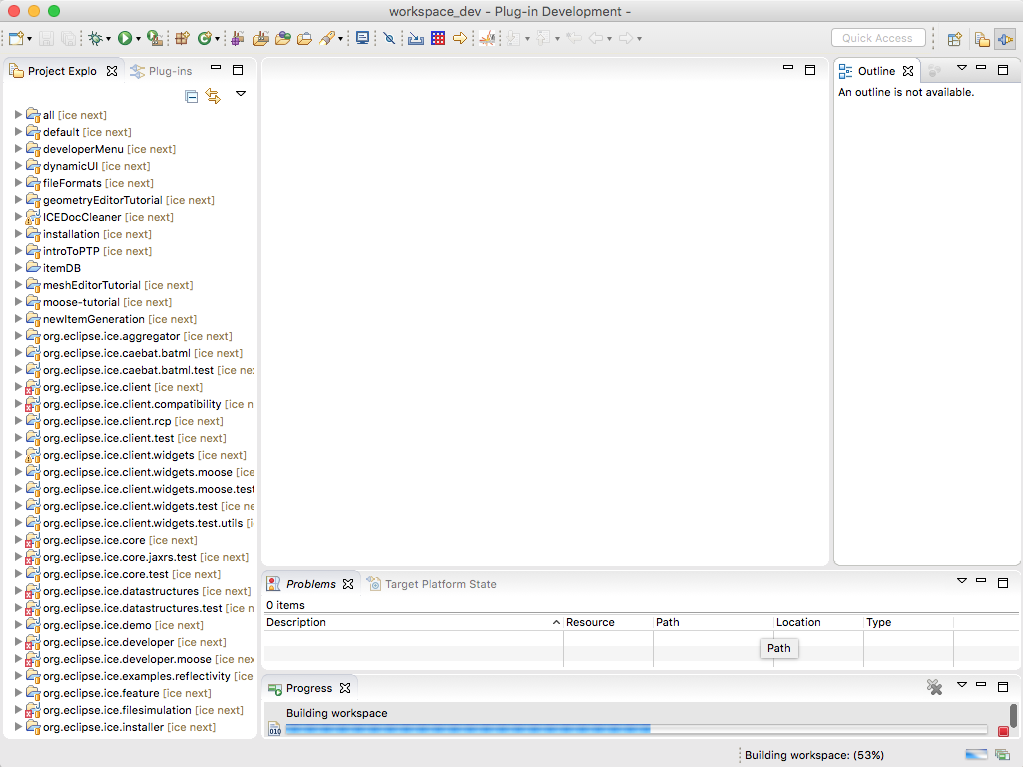
\includegraphics[width=\textwidth]{figures/cloned} \end{center}
